\chapter{\IfLanguageName{dutch}{proof-of-concept}{proof-of-concept}}%
\label{ch:proof-of-concept}
\section{Inleiding}
In dit hoofdstuk bespreken we de implementatie van het proof-of-concept. We zullen elke fase van het proces in detail bespreken en de implementatie van de bijbehorende componenten toelichten. Hierbij zullen we ook de uitkomsten van elke fase beschrijven en hoe deze kunnen gebruikt worden in de volgende fase. \\

\section{Webscraper}
\subsection{Algemene Eisen}
Binnen de algemene eisen zal de webscraper voldoen aan de ethische aspecten \ref{subsection:scraper-ethische-aspecten} die zijn beschreven in de state of the art van dit onderzoek. Dit betekent dat de scraper de regels en richtlijnen van de gescrapte websites zal respecteren en zich zal houden aan eventuele beperkingen zoals vermeld in het robots.txt-bestand. Hierdoor wordt ervoor gezorgd dat de scrapingactiviteiten op een ethisch verantwoorde manier worden uitgevoerd. \\

Daarnaast zal de webscraper in staat zijn om verschillende websites te scrapen, met de focus op het verzamelen van de frontpage-inhoud. Specifiek zal de scraper de eerste 20 items van de frontpage van elke website verzamelen. \\

De webscraper zal twee bekende nieuwsbronnen scrapen, namelijk HLN en DeMorgen.

\subsection{Verkenning}
Alvorens we de webscraper kunnen implementeren, is het nodig om de DOM van beide websites te bekijken en een patroon hierin te herkennen. \\
\subsubsection{HLN}
Op de startpagina van HLN kunnen we zien (figuur \ref{fig:hln_frontpage}) dat elk nieuwsartikel zich bevindt binnen een article-tag bevindt. De eerste subtag is een a-tag met hierin de href naar het artikel. \\ Deze href zal belangrijk zijn om de datum te valideren en de titel te extraheren. We moeten deze dus opslaan. 

\begin{center}
    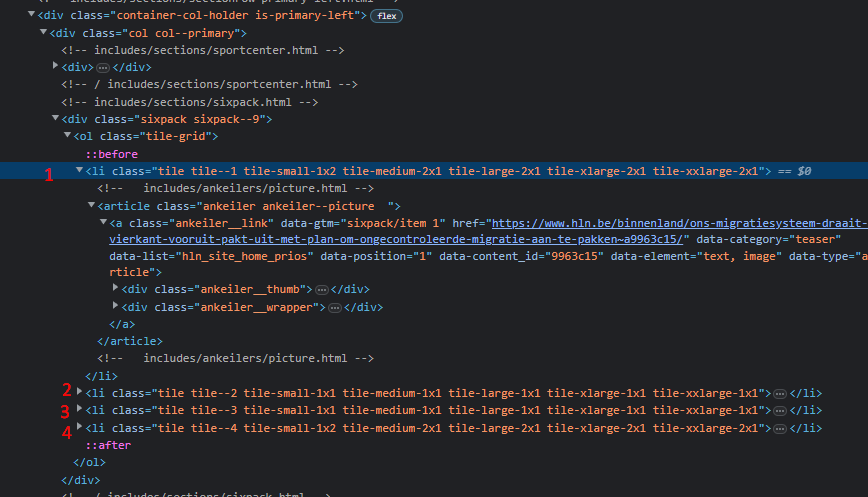
\includegraphics[width = 6in]{hln_frontpage2.png}
    \captionof{figure}{DOM van de startpagina van HLN met aangeduide nieuwsartikels.}
    \label{fig:hln_frontpage}
\end{center}

Als we vervolgens gaan kijken naar de DOM van een artikel, zien we dat de titel weergegeven wordt binnen een header-tag met als class 'article\_\_header' deze titel heeft als class 'article\_\_title'. De datum wordt weergegeven binnen een time-tag met datetime als value en class 'article\_\_time'. De datum is ook opgemaakt in een bepaald formaat, dd-mm-yy, hh:mm. Deze gegevens zijn essentieel voor de scraper. In figuur \ref{fig:hln_article} vind je dit terug. \\

\begin{center}
    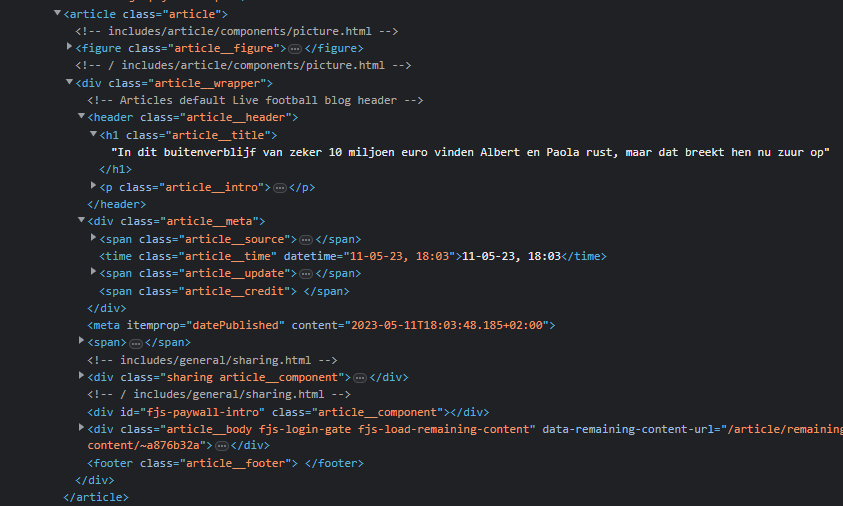
\includegraphics[width = 6in]{hln_article1.png}
    \captionof{figure}{DOM van een artikel op HLN met de essentiële elementen gemarkeerd.}
    \label{fig:hln_article}
\end{center}

\subsubsection{De Morgen}
De structuur van de artikels op de startpagina van De Morgen is vergelijkbaar met die van HLN. Zoals te zien is in figuur \ref{fig:demorgen_frontpage}, worden de artikels ook weergegeven binnen een article-tag, waarbij de eerste subtag een a-tag is.

\begin{center}
    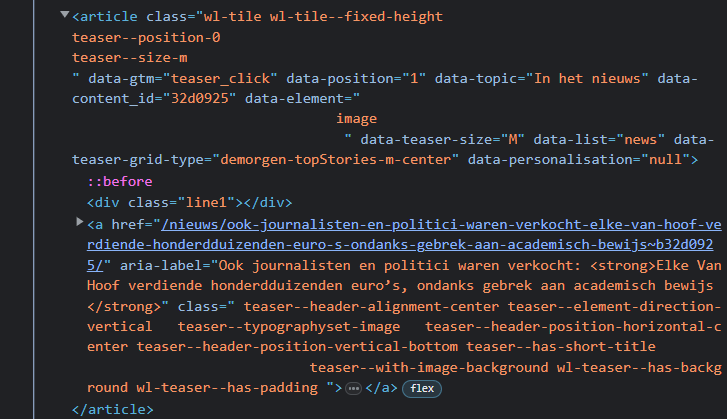
\includegraphics[width = 6in]{demorgen_frontpage2.png}
    \captionof{figure}{DOM van een artikel op De Morgen.}
    \label{fig:demorgen_frontpage}
\end{center}

Bij het doorklikken op een willekeurig artikel zien we dat de DOM vergelijkbaar is, maar niet exact hetzelfde qua structuur. In figuur \ref{fig:demorgen_article} zie je de DOM.

\begin{center}
    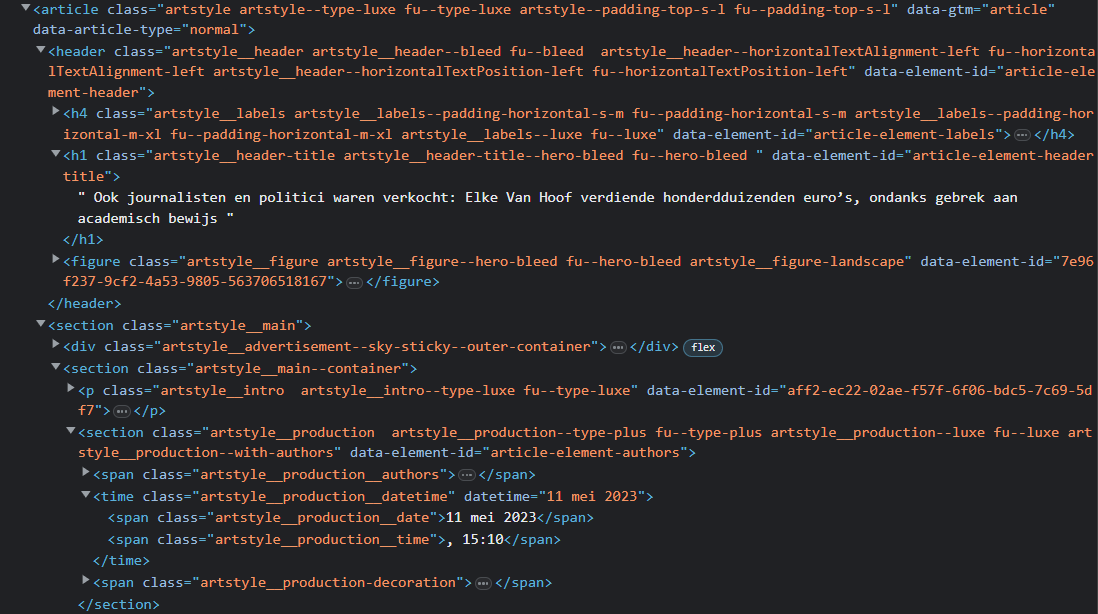
\includegraphics[width = 6in]{demorgen_article.png}
    \captionof{figure}{DOM van een artikel op De Morgen.}
    \label{fig:demorgen_article}
\end{center}

Nu dat we deze informatie hebben. Kunnen we beginnen aan de implementatie van de scraper. 




\subsection{Implementatie}

\subsection{Uitkomst}
Deze uitkomst zal gebruikt worden binnen volgende fase ...  \\

\section{GPT}
\subsection{Inleiding}
Praten over prompten
\subsection{Implementatie}
jjj
\subsection{Uitkomst}
vertellen wat de uitkomst is van de prompts, en dat we dit nu kunnen gebruiken om een schilderij te genereren.

\section{DALL-E}
\subsection{Inleiding}
Kort nog eens de moeilijkheden uitleggen (interpretatie etc.)
\subsection{Implementatie}
Kort uitleggen
\subsection{Resultaat}
...
\begin{listing}[H]
\begin{minted}[breaklines, style=solarized-dark]{python}
   # This is a random comment
   class Yo:
        def fn:
            return 1337
   
  print(``yo'')
  
\end{minted}
\caption{Test code format}
\end{listing}